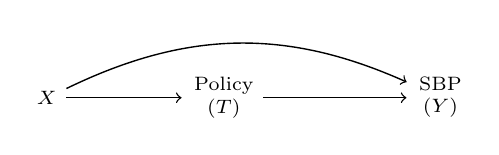
\begin{tikzpicture}[shorten > = 1pt, line width=0.5pt, font=\scriptsize]
\fontfamily(roboto)
\tikzstyle{every node} = [rectangle, fill=white, draw=none]
\node (x) at (0,0) [align=center] {$X$};
\node (t) at  (2.25,0) [align=center] {Policy\\($T$)};
\node (y) at  (5,0) [align=center] {SBP\\($Y$)};
\foreach \from/\to in {x/t, t/y}
  \draw [->] (\from) -- (\to);
\draw [->] (x) to [bend left=25] (y);
\end{tikzpicture}